\chapter{The NED Language}
\label{cha:the-ned-language}


\section{NED Overview}

The user describes the structure of a simulation model in the NED language. NED
stands for Network Description. NED lets the user declare simple modules, and
connect and assemble them into compound modules. The user can label some compound
modules as \textit{networks}, self-contained simulation models. Channels are
another component type, whose instances can also be used in compound modules.

The NED language has several features which let it scale well to large projects:

\begin{description}

\item[Hierarchical] The traditional way to deal with complexity is via
introducing hierarchies. In {\opp}, any module which would be too complex as
a single entity can be broken down into smaller modules, and used as a
compound module.

\item[Component-Based] Simple modules and compound modules are inherently
reusable, which not only reduces code copying, but more importantly, allows
component libraries (like the INET Framework, MiXiM, Castalia, etc.) to
exist.

\item[Interfaces] Module and channel interfaces can be used as a
placeholder where normally a module or channel type would be used, and the
concrete module or channel type is determined at network setup time by a
parameter. Concrete module types have to ``implement'' the interface they
can substitute. For example, given a compound module type named
\ttt{MobileHost} contains a \ttt{mobility} submodule of the type
\ttt{IMobility} (where \ttt{IMobility} is a module interface), the actual
type of \ttt{mobility} may be chosen from the module types that implemented
\ttt{IMobility} (\ttt{RandomWalkMobility}, \ttt{TurtleMobility}, etc.)

\item[Inheritance] Modules and channels can be subclassed. Derived modules
and channels may add new parameters, gates, and (in the case of compound
modules) new submodules and connections. They may set existing parameters
to a specific value, and also set the gate size of a gate vector. This
makes it possible, for example, to take a \ttt{GenericTCPClientApp} module
and derive an \ttt{FTPClientApp} from it by setting certain parameters to a fixed
value; or to derive a \ttt{WebClientHost} compound module from a
\ttt{BaseHost} compound module by adding a \ttt{WebClientApp} submodule and
connecting it to the inherited \ttt{TCP} submodule.

\item[Packages] The NED language features a Java-like package structure,
to reduce the risk of name clashes between different models. \ttt{NEDPATH}
(similar to Java's \ttt{CLASSPATH}) was also introduced to make it easier
to specify dependencies among simulation models.

\item[Inner types] Channel types and module types used locally by a
compound module can be defined within the compound module, in order to
reduce namespace pollution.

\item[Metadata annotations] It is possible to annotate module or channel
types, parameters, gates and submodules by adding properties. Metadata are
not used by the simulation kernel directly, but they can carry extra
information for various tools, the runtime environment, or even for other
modules in the model. For example, a module's graphical representation
(icon, etc)  or the prompt string and measurement unit (milliwatt, etc) of a
parameter are already specified as metadata annotations.

\end{description}

\begin{note}
    The NED language has changed significantly in the 4.0 version.
    Inheritance, interfaces, packages, inner types, metadata annotations, inout
    gates were all added in the 4.0 release, together with many other features.
    Since the basic syntax has changed as well, old NED files need to be
    converted to the new syntax. There are automated tools for this purpose, so
    manual editing is only needed to take advantage of new NED features.
\end{note}

The NED language has an equivalent tree representation which can be
serialized to XML; that is, NED files can be converted to XML and back
without loss of data, including comments. This lowers the barrier for
programmatic manipulation of NED files, for example extracting information,
refactoring and transforming NED, generating NED from information stored in
other system like SQL databases, and so on.

\begin{note}
    This chapter is going to explain the NED language gradually, via examples.
    If you are looking for a more formal and concise treatment, see
    Appendix \ref{cha:ned-language-grammar}.
\end{note}


\section{Warmup}
\label{sec:ch-ned-lang:warmup}

In this section we introduce the NED language via a complete and
reasonably real-life example: a communication network.

Our hypothetical network consists of nodes. One each node there's an
application running which generates packets at random intervals.
The nodes are routers themselves as well. We assume that the application
uses datagram-based communication, so that we can leave out the
transport layer from the model.


\subsection{The Network}
\label{sec:ch-ned-lang:warmup:network}

First we'll define the network, then in the next sections we'll continue
to define the network nodes.

Let the network topology be as in Figure \ref{fig:ned-routing-topology}.

\begin{figure}[htbp]
  \centering
  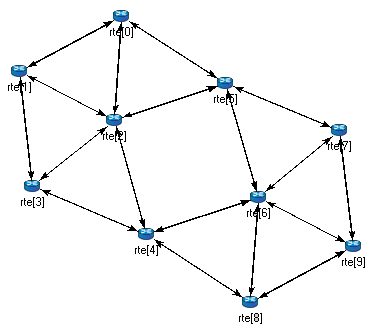
\includegraphics[scale=0.6]{figures/ned-routing-network}
  \caption{The network}
  \label{fig:ned-routing-topology}
\end{figure}

The corresponding NED description would look like this:

\begin{ned}
//
// A network
//
network Network
{
    submodules:
        node1: Node;
        node2: Node;
        node3: Node;
        ...
    connections:
        node1.port++ <--> {datarate=100Mbps;} <--> node2.port++;
        node2.port++ <--> {datarate=100Mbps;} <--> node4.port++;
        node4.port++ <--> {datarate=100Mbps;} <--> node6.port++;
        ...
}
\end{ned}

The above code defines a network type named \ttt{Network}. Note that the NED
language uses the familiar curly brace syntax, and ``\ttt{//}'' to denote
comments.

\begin{note}
    Comments in NED not only make the source code more readable, but in the
    {\opp} IDE they also get displayed at various places (tooltips, content
    assist, etc), and become part of the documentation extracted from the NED
    files. The NED documentation system, not unlike \textit{JavaDoc} or
    \textit{Doxygen}, will be described in Chapter \ref{cha:neddoc}.
\end{note}

The network contains several nodes, named \ttt{node1}, \ttt{node2}, etc.
from the NED module type \ttt{Node}. We'll define \ttt{Node} in the next
sections.

The second half of the declaration defines how the nodes are to be
connected. The double arrow means bidirectional connection. The connection
points of modules are called gates, and the \ttt{port++} notation adds a
new gate to the \ttt{port[]} gate vector. Gates and connections will be
covered in more detail in sections \ref{sec:ch-ned-lang:gates} and
\ref{sec:ch-ned-lang:connections}. Nodes are connected with a channel that
has a data rate of 100Mbps.

\begin{note}
    In many other systems, the equivalent of {\opp} gates are called
    \textit{ports}. We have retained the term \textit{gate} to reduce
    collisions with other uses of the otherwise overloaded word
    \textit{port}: router port, TCP port, I/O port, etc.
\end{note}

The above code would be placed into a file named \ttt{Net6.ned}. It is
a convention to put every NED definition into its own file and to name the
file accordingly, but it is not mandatory to do so.

One can define any number of networks in the NED files, and for every
simulation the user has to specify which network he wants to set up.
The usual way of specifying the network is to put the \fconfig{network}
option into the configuration (by default the \ffilename{omnetpp.ini} file):

\begin{inifile}
[General]
network = Network
\end{inifile}


\subsection{Introducing a Channel}

It is cumbersome to have to repeat the data rate for every connection.
Luckily, NED provides a convenient solution: one can create a new channel
type that encapsulates the data rate setting, and this channel type can
be defined inside the network so that it does not litter the global
namespace.

The improved network will look like this:

\begin{ned}
//
// A Network
//
network Network
{
    types:
        channel C extends ned.DatarateChannel {
            datarate = 100Mbps;
        }
    submodules:
        node1: Node;
        node2: Node;
        node3: Node;
        ...
    connections:
        node1.port++ <--> C <--> node2.port++;
        node2.port++ <--> C <--> node4.port++;
        node4.port++ <--> C <--> node6.port++;
        ...
}
\end{ned}

Later sections will cover the concepts used (inner types, channels, the
\ttt{DatarateChannel} built-in type, inheritance) in details.


\subsection{The App, Routing and Queue Simple Modules}

Simple modules are the basic building blocks for other (compound) modules.
All active behavior in the model is encapsulated in simple modules.
Behavior is defined with a C++ class; NED files only declare the externally
visible interface of the module (gates, parameters).

In our example, we could define \ttt{Node} as a simple module. However,
its functionality is quite complex (traffic generation, routing, etc),
so it is better to implement it with several smaller simple module types
which we are going to assemble into a compound module. We'll have
one simple module for traffic generation (\ttt{App}), one for routing
(\ttt{Routing}), and one for queueing up packets to be sent out (\ttt{Queue}).
For brevity, we omit the bodies of the latter two in the code below.

\begin{ned}
simple App
{
    parameters:
        int destAddress;
        ...
        @display("i=block/browser");
    gates:
        input in;
        output out;
}

simple Routing
{
    ...
}

simple Queue
{
    ...
}
\end{ned}

By convention, the above simple module declarations go into the
\ttt{App.ned}, \ttt{Routing.ned} and \ttt{Queue.ned} files.

\begin{note}
    Note that module type names (\ttt{App}, \ttt{Routing}, \ttt{Queue})
    begin with a capital letter, and parameter and gate names begin with
    lowercase -- this is the recommended naming convention. Capitalization
    matters because the language is case sensitive.
\end{note}

Let us see the first simple module type declaration. \ttt{App} has a
parameter called \ttt{destAddress} (others have been omitted for now),
and two gates named \ttt{out} and \ttt{in} for sending and receiving
application packets.

The argument of \fprop{@display()} is called a \textit{display string},
and it defines the rendering of the module in graphical environments;
\ttt{"i=..."} defines the default icon.

Generally, \ttt{@}-words like \ttt{@display} are called \textit{properties}
in NED, and they are used to annotate various objects
with metadata. Properties can be attached to files, modules, parameters, gates,
connections, and other objects, and parameter values have a very flexible
syntax.


\subsection{The Node Compound Module}

Now we can assemble \ttt{App}, \ttt{Routing} and {Queue} into the
compound module \ttt{Node}. A compound module can be thought of as
a ``cardboard box'' that groups other modules into a larger unit,
which can further be used as a building block for other modules;
networks are also a kind of compound module.

\begin{figure}[htbp]
  \centering
  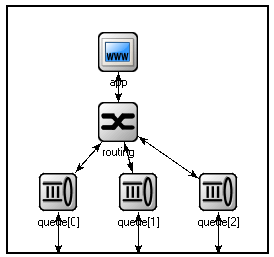
\includegraphics[scale=0.6]{figures/ned-routing-node}
  \caption{The Node compound module}
  \label{fig:ned-routing-node}
\end{figure}

\begin{ned}
module Node
{
    parameters:
        @display("i=misc/node_vs,gold");
    gates:
        inout port[];
    submodules:
        app: App;
        routing: Routing;
        queue[sizeof(port)]: Queue;
    connections:
        routing.localOut --> app.in;
        routing.localIn <-- app.out;
        for i=0..sizeof(port)-1 {
            routing.out[i] --> queue[i].in;
            routing.in[i] <-- queue[i].out;
            queue[i].line <--> port[i];
        }
}
\end{ned}

Compound modules, like simple modules, may have parameters and gates.
Our \ttt{Node} module contains an \ttt{address} parameter, plus a
\textit{gate vector} of unspecified size, named \ttt{port}.
The actual gate vector size will be determined implicitly by the number
of neighbours when we create a network from nodes of this type.
The type of \ttt{port[]} is \ttt{inout}, which allows bidirectional
connections.

The modules that make up the compound module are listed under
\fkeyword{submodules}. Our \ttt{Node} compound module type has an \ttt{app} and
a \ttt{routing} \textit{submodule}, plus a \ttt{queue[]} \textit{submodule
vector} that contains one \ttt{Queue} module for each port, as specified by
\ttt{[sizeof(port)]}. (It is legal to refer to \ttt{[sizeof(port)]} because
the network is built in top-down order, and the node is already created and
connected at network level when its submodule structure is built out.)

In the \fkeyword{connections} section, the submodules are connected to each
other and to the parent module. Single arrows are used to connect input and
output gates, and double arrows connect inout gates, and a \fkeyword{for} loop
is utilized to connect the \ttt{routing} module to each \ttt{queue} module, and
to connect the outgoing/incoming link (\ttt{line} gate) of each queue to the
corresponding port of the enclosing module.


\subsection{Putting It Together}

We have seen all NED definitions, but how does it get used by {\opp}? When
the simulation program is started, it loads the NED files. The program
should already contain the C++ classes that implement the needed simple
modules, \ttt{App}, \ttt{Routing} and \ttt{Queue}; their C++ code is either
part if the executable or gets loaded from shared library. The simulation
program also loads the configuration (\ffilename{omnetpp.ini}), and determines
from it that the simulation model to be run is the \ttt{Network} network.
Then the network gets instantiated for simulation.

The simulation model is built in a top-down preorder fashion. This means
that starting from an empty system module, all submodules are created,
their parameters and gate vector sizes get assigned and they get fully connected
before proceeding to go into the submodules to build their internals.

\bigskip
\begin{center}
* * *
\end{center}
\bigskip

In the following sections we'll go through the elements of the NED
language and look at them in more details.



\section{Simple Modules}
\label{sec:ch-ned-lang:simple-modules}

Simple modules are the active components in the model.
Simple modules are defined with the \fkeyword{simple} keyword.

An example simple module:

\begin{ned}
simple Queue
{
    parameters:
        int capacity;
        @display("i=block/queue");
    gates:
        input in;
        output out;
}
\end{ned}

Both the \fkeyword{parameters} and \fkeyword{gates} sections are optional, that is,
they can be left out if there's no parameter or gate. In addition, the
\fkeyword{parameters} keyword itself is optional too, it can be left out
even if there are parameters or properties.

Note that the NED definition doesn't contain any code to define the
operation of the module: that part is expressed in C++. By default, {\opp}
looks for C++ classes of the same name as the NED type (so here, \ttt{Queue}).

One can explicitly specify the C++ class with the \fprop{@class} property.
Classes with namespace qualifiers are also accepted, as shown in the following
example that uses the \ttt{mylib::Queue} class:

\begin{ned}
simple Queue
{
    parameters:
        int capacity;
        @class(mylib::Queue);
        @display("i=block/queue");
    gates:
        input in;
        output out;
}
\end{ned}

If you have several modules that are all in a common namespace, then a
better alternative to \fprop{@class} is the \fprop{@namespace} property. The
C++ namespace given with \fprop{@namespace} will be prepended to the normal
class name. In the following example, the C++ classes will be
\ttt{mylib::App}, \ttt{mylib::Router} and \ttt{mylib::Queue}:

\begin{ned}
@namespace(mylib);

simple App {
   ...
}

simple Router {
   ...
}

simple Queue {
   ...
}
\end{ned}

As you've seen, \fprop{@namespace} can be specified on file level. Moreover,
when placed in a file called \ttt{package.ned}, the namespace will apply to
all files in the same directory and all directories below.

The implementation C++ classes need to be subclassed from the
\cclass{cSimpleModule} library class; chapter \ref{cha:simple-modules} of
this manual describes in detail how to write them.

Simple modules can be extended (or specialized) via subclassing. The
motivation for subclassing can be to set some open parameters or gate sizes
to a fixed value (see \ref{sec:ch-ned-lang:parameters} and
\ref{sec:ch-ned-lang:gates}), or to replace the C++ class with a different
one. Now, by default the derived NED module type will \textit{inherit} the
C++ class from its base, so it is important to remember that you need to
write out \fprop{@class} if you want it to use the new class.

The following example shows how to specialize a module by setting a parameter
to a fixed value (and leaving the C++ class unchanged):

\begin{ned}
simple Queue
{
   int capacity;
   ...
}

simple BoundedQueue extends Queue
{
   capacity = 10;
}
\end{ned}

In the next example, the author wrote a \ttt{PriorityQueue} C++ class, and
wants to have a corresponding NED type, derived from \ttt{Queue}. However,
it does not work as expected:

\begin{ned}
simple PriorityQueue extends Queue // wrong! still uses the Queue C++ class
{
}
\end{ned}

The correct solution is to add a \fprop{@class} property to override the
inherited C++ class:

\begin{ned}
simple PriorityQueue extends Queue
{
   @class(PriorityQueue);
}
\end{ned}

Inheritance in general will be discussed in section \ref{sec:ch-ned-lang:inheritance}.



\section{Compound Modules}
\label{sec:ch-ned-lang:compound-modules}

A compound module groups other modules into a larger unit. A compound
module may have gates and parameters like a simple module, but no active
behavior is associated with it.\footnote{Although the C++ class
for a compound module can be overridden with the \fprop{@class} property,
this is a feature that should probably never be used. Encapsulate the code
into a simple module, and add it as a submodule.}

\begin{note}
    When there is a temptation to add code to a compound module,
    then encapsulate the code into a simple module, and add it as
    a submodule.
\end{note}

A compound module declaration may contain several sections,
all of them optional:

\begin{ned}
module Host
{
   types:
       ...
   parameters:
       ...
   gates:
       ...
   submodules:
       ...
   connections:
       ...
}
\end{ned}

Modules contained in a compound module are called submodules, and they are
listed in the \ttt{submodules} section. One can create arrays of submodules
(i.e. submodule vectors), and the submodule type may come from a parameter.

Connections are listed under the \ttt{connections} section of the
declaration. One can create connections using simple programming constructs
(loop, conditional). Connection behaviour can be defined by associating a
channel with the connection; the channel type may also come from a
parameter.

Module and channel types only used locally can be defined in the
\ttt{types} section as inner types, so that they don't pollute the
namespace.

Compound modules may be extended via subclassing. Inheritance may add new
submodules and new connections as well, not only parameters and gates;
also, one may refer to inherited submodules, to inherited types etc. What
is not possible is to "de-inherit" submodules or connections, or to modify
inherited ones.

In the following example, we show how one can assemble common protocols
into a "stub" for wireless hosts, and add user agents via
subclassing.\footnote{Module types, gate names, etc. used in the example
are fictional, not based on an actual {\opp}-based model framework}

\begin{ned}
module WirelessHostBase
{
   gates:
       input radioIn;
   submodules:
       tcp: TCP;
       ip: IP;
       wlan: Ieee80211;
   connections:
       tcp.ipOut --> ip.tcpIn;
       tcp.ipIn <-- ip.tcpOut;
       ip.nicOut++ --> wlan.ipIn;
       ip.nicIn++ <-- wlan.ipOut;
       wlan.radioIn <-- radioIn;
}

module WirelessUser extends WirelessHostBase
{
   submodules:
       webAgent: WebAgent;
   connections:
       webAgent.tcpOut --> tcp.appIn++;
       webAgent.tcpIn <-- tcp.appOut++;
}
\end{ned}

The \ttt{WirelessUser} compound module can further be extended,
for example with an Ethernet port:

\begin{ned}
module DesktopUser extends WirelessUser
{
   gates:
       inout ethg;
   submodules:
       eth: EthernetNic;
   connections:
       ip.nicOut++ --> eth.ipIn;
       ip.nicIn++ <-- eth.ipOut;
       eth.phy <--> ethg;
}
\end{ned}



\section{Channels}
\label{sec:ch-ned-lang:channels}

Channels encapsulate parameters and behaviour associated with connections.
Channels are like simple modules, in the sense that there are C++ classes
behind them. The rules for finding the C++ class for a NED channel type is
the same as with simple modules: the default class name is the NED type
name unless there is a \fprop{@class} property (\fprop{@namespace} is also
observed), and the C++ class is inherited when the channel is subclassed.

Thus, the following channel type would expect a \ttt{CustomChannel} C++ class
to be present:

\begin{ned}
channel CustomChannel  // needs a CustomChannel C++ class
{
}
\end{ned}

The practical difference to modules is that you rarely need to write you own
channel C++ class, because there are predefined channel types that you can
subclass from, inheriting their C++ code. The predefined types are:
\ttt{ned.IdealChannel}, \ttt{ned.Delay\-Channel} and \ttt{ned.Datarate\-Channel}.
(``\ttt{ned}'' is the package name; you can get rid of it if you import the types
with the \ttt{import ned.*} or similar directive. Packages and imports
are described in section \ref{sec:ch-ned-lang:packages}.)

\ttt{IdealChannel} has no parameters, and lets through all messages without
delay or any side effect. A connection without a channel object
and a connection with an \ttt{IdealChannel} behave in the same way.
Still, \ttt{IdealChannel} has its uses, for example when a channel object
is required so that it can carry a new property or parameter that is
going to be read by other parts of the simulation model.

\ttt{DelayChannel} has two parameters:

\begin{itemize}
    \item \ttt{delay} is a \ttt{double} parameter which represents the
          propagation delay of the message. Values need to be specified
          together with a time unit (\ttt{s}, \ttt{ms}, \ttt{us}, etc.)
    \item \ttt{disabled} is a boolean parameter that defaults to \ttt{false};
          when set to \ttt{true}, the channel object will drop all messages.
\end{itemize}

\ttt{DatarateChannel} has a few additional parameters compared to \ttt{DelayChannel}:

\begin{itemize}
    \item \ttt{datarate} is a \ttt{double} parameter that represents the
          data rate of the channel. Values need to be specified
          in bits per second or its multiples as unit (\ttt{bps},
          \ttt{Kbps}, \ttt{Mbps}, \ttt{Gbps}, etc.) Zero is treated
          specially and results in zero transmission duration, i.e.
          it stands for infinite bandwidth. Zero is also the default.
          Data rate is used for calculating the transmission duration of
          packets.
    \item \ttt{ber} and \ttt{per} stand for Bit Error Rate and Packet Error Rate,
          and allow basic error modelling. They expect a \ttt{double}
          in the $[0,1]$ range. When the channel decides (based on random
          numbers) that an error occurred during transmission a packet,
          it sets an error flag in the packet object. The receiver
          module is expected to check the flag, and discard the packet
          as corrupted if it is set. The default \ttt{ber} and \ttt{per}
          are zero.
\end{itemize}

\begin{note}
    There is no channel parameter that would decide whether the channel
    delivers the message object to the destination module at the end or
    at the start of the reception; that is decided by the C++ code
    of the target simple module. See the \ffunc{setDeliverOn\-Reception\-Start()}
    method of \cclass{cGate}.
\end{note}

The following example shows how to create a new channel type by
specializing \ttt{DatarateChannel}:

\begin{ned}
channel C extends ned.DatarateChannel
{
    datarate = 100Mbps;
    delay = 100us;
    ber = 1e-10;
}
\end{ned}

\begin{note}
    The three built-in channel types are also used for connections where
    the channel type not explicitly specified.
\end{note}

You may add parameters and properties to channels via subclassing, and
modify existing ones. In the following example, we introduce length-based
calculation of the propagation delay:

\begin{ned}
channel DatarateChannel2 extends ned.DatarateChannel
{
    double length @unit(m);
    delay = this.length / 200000km * 1s;
}
\end{ned}

Parameters are primarily useful as input to the underlying C++ class, but
even if you reuse the underlying C++ class of built-in channel types, they
may be read and used by other parts of the model. For example, adding a
\ttt{cost} parameter (or \fprop{@cost} property) may be observed by the
routing algorithm and used for routing decisions. The following example
shows a \ttt{cost} parameter, and annotation using a property
(\fprop{@backbone}).

\begin{ned}
channel Backbone extends ned.DatarateChannel
{
    @backbone;
    double cost = default(1);
}
\end{ned}



\section{Parameters}
\label{sec:ch-ned-lang:parameters}

Parameters are variables that belong to a module. Parameters can be
used in building the topology (number of nodes, etc), and to supply
input to C++ code that implements simple modules and channels.

Parameters can be of type \fkeyword{double}, \fkeyword{int},
\fkeyword{bool}, \fkeyword{string} and \fkeyword{xml}; they can also
be declared \fkeyword{volatile}. For the numeric types, a unit of
measurement can also be specified (\fprop{@unit} property), to increase
type safety.

Parameters can get their value from NED files or from the configuration
(\ffilename{omnetpp.ini}). A default value can also be given (\ttt{default(}...\ttt{)}),
which gets used if the parameter is not assigned otherwise.

Let us see an example before we go into details:

\begin{ned}
simple App
{
    parameters:
        int address;  // local node address
        string destAddresses;  // destination addresses
        volatile double sendIaTime @unit(s) = default(exponential(1s));
                               // time between generating packets
        volatile int packetLength @unit(byte);  // length of one packet
    ...
}
\end{ned}

%% XXX explain the example


\subsubsection{Values}

Parameters may get their values from several places: from NED code, from
the configuration (\ffilename{omnetpp.ini}), or even, interactively from the
user.

The following example shows how parameters of an \ttt{App} module (from the
previous example) may be assigned when \ttt{App} gets used as a submodule:

\begin{ned}
module Node
{
    submodules:
        app : App {
            sendIaTime = 3s;
            packetLength = 1024B; // B=byte
        }
        ...
}
\end{ned}

After the above definition, the \ttt{app} submodule's parameters cannot
be changed from \ffilename{omnetpp.ini} any more.

\begin{important}
    A value assigned in NED cannot be overwritten from ini files; they
    count as "hardcoded" as far as ini files are concerned.
\end{important}

Provided that the value isn't set in the NED file, a parameter can be assigned
in the configuration in the following way:

\begin{inifile}
**.sendIaTime = 100ms
\end{inifile}

The above line applies to all parameters called \ttt{sendIaTime}, whichever
module they belong to; it is possible to write more selective assignments
by replacing \ttt{**} with more specific patterns. Parameter assignments in
the configuration are described in section
\ref{sec:ch-config-sim:parameter-settings}.

One can also write expressions, including stochastic expressions, in the ini file:

\begin{inifile}
**.sendIaTime = 2s + exponential(100ms)
\end{inifile}

If there is no assignment in the ini file, the default value (given with
\ttt{=default(...)} in NED) is applied implicitly. If there is no default
value, the user will be asked, provided the simulation program is allowed
to do that; otherwise there will be an error. (Interactive mode is
typically disabled for batch executions where it would do more harm than
good.)

It is also possible to explicitly apply the default (this can sometimes
be useful):

\begin{inifile}
**.sendIaTime = default
\end{inifile}

Finally, one can explicitly ask the simulator to prompt the user interactively
for the value (again, provided that interactivity is enabled, otherwise
this will result in an error):

\begin{inifile}
**.sendIaTime = ask
\end{inifile}

\begin{note}
    How do you decide whether to assign a parameter from NED or from an ini
    file? The point of ini files is a cleaner separation of the \textit{model}
    and \textit{experiments}. NED files (together with C++ code) are considered
    to be part of the model, and to be more or less constant. Ini files, on
    the other hand, are for experimenting with the model, by running it
    several times with different parameters. Thus, parameters that are expected
    to change (or make sense to be changed) during experimentation should be
    put into ini files.
\end{note}


\subsubsection{Expressions}

Parameter values may be given with expressions. NED language expressions
have a C-like syntax, with some variations on operator names: binary and
logical XOR are \ttt{\#} and \ttt{\#\#}, while \ttt{\^} has been reassigned
to \textit{power-of} instead. The \ttt{+} operator does string
concatenation as well as numeric addition. Expressions can use various
numeric, string, stochastic and other functions (\ttt{fabs()}, \ttt{toUpper()},
\ttt{uniform()}, \ttt{erlang\_k()}, etc.).

\begin{note}
    The list of NED functions can be read in Appendix \ref{cha:ned-functions}.
    The user can also extend NED with new functions.
\end{note}

%% XXX also sources of random numbers

Expressions may refer to module parameters, gate vector and module vector sizes
(using the \fkeyword{sizeof} operator) and the index of the current module
in a submodule vector (\fkeyword{index}).

%% XXX note: fullPath() etc functions!

A Expressions may refer to parameters of the compound module being defined,
of the current module (with the \ttt{this.} prefix), and to parameters
of already defined submodules, with the syntax \ttt{submodule.parametername}
(or \ttt{submodule[index].parametername}).

%% XXX example: address = address;  delay=this.distance/this.speed;

%% XXX there are no parameter arrays, but... demonstrate the choose() function


\subsubsection{volatile}

The \fkeyword{volatile} modifier causes the parameter's value expression to
be evaluated every time the parameter is read. This has significance if the
expression is not constant, for example it involves numbers drawn from a
random number generator. In contrast, non-volatile parameters are evaluated
only once. (This practically means that they are evaluated and replaced
with the resulting constant at the start of the simulation.)

To better understand \fkeyword{volatile}, let's suppose we have an
\ttt{ActiveQueue} simple module that has a \ttt{volatile double} parameter
named \ttt{serviceTime}.

The queue module's C++ implementation would re-read the \ttt{serviceTime}
parameter at runtime for every job serviced; so if \ttt{serviceTime} is
assigned an expression like \ttt{uniform(0.5s, 1.5s)}, every job would have
a different, random service time.

In practice, a volatile parameter usually means that the underlying C++
code will re-read the parameter every time a value is needed at runtime, so
the parameter can be used a source of random numbers.

\begin{note}
    This does not mean that a non-volatile parameter cannot be assigned a value
    like \ttt{uniform(0.5s, 1.5s)}. It can, but that has a totally different
    effect. Had we omitted the \ttt{volatile} keyword from the
    \ttt{serviceTime} parameter, for example, the effect would be that every
    job had the \textit{same} constant service time, say \ttt{1.2975367s},
    chosen randomly at the beginning of the simulation.
\end{note}

\subsubsection{Units}

One can declare a parameter to have an associated unit of measurement,
by adding the \fprop{@unit} property. An example:

\begin{ned}
simple App
{
    parameters:
        volatile double sendIaTime @unit(s) = default(exponential(350ms));
        volatile int packetLength @unit(byte) = default(4KB);
    ...
}
\end{ned}

The \ttt{@unit(s)} and \ttt{@unit(byte)} bits declare the measurement unit
for the parameter. Values assigned to parameters must have the same or
compatible unit, i.e. \ttt{@unit(s)} accepts milliseconds, nanoseconds,
minutes, hours, etc., and \ttt{@unit(byte)} accepts kilobytes, megabytes,
etc. as well.

\begin{note}
    The list of units accepted by {\opp} is listed in the Appendix, see
    \ref{ch-ned-ref:sec:units}. Unknown units (\ttt{bogomips}, etc.)
    can also be used, but there are no conversions for them,
    i.e. decimal prefixes will not be recognized.
\end{note}

The {\opp} runtime does a full and rigorous unit check on
parameters to ensure ``unit safety'' of models. Constants should
always include the measurement unit.

The \fprop{@unit} property of a parameter cannot be added or overridden
in subclasses or in submodule declarations.


\subsubsection{XML Parameters}

Sometimes modules need more complex input than simple module parameters
can describe. Then you'd put these parameters into an external config file,
and let the modules read and process the file. You'd pass the file name
to the modules in a string parameter.

These days, XML is increasingly becoming a standard format for configuration
files as well, so you might as well describe your configuration in XML.
From the 3.0 version, {\opp} contains built-in support for XML config files.

{\opp} wraps the XML parser (LibXML, Expat, etc.), reads and DTD-validates
the file (if the XML document contains a DOCTYPE), caches the file
(so that if you refer to it from several modules, it'll still be loaded
only once), lets you pick parts of the document via an XPath-subset notation,
and presents the contents to you in a DOM-like object tree.

This machinery can be accessed via the NED parameter type \ttt{xml}, and the
\ttt{xmldoc()} operator. You can point \ttt{xml}-type module parameters
to a specific XML file (or to an element inside an XML file) via the
\ttt{xmldoc()} operator. You can assign \ttt{xml} parameters both from NED
and from \ffilename{omnetpp.ini}.

The following example declares an \ttt{xml} parameter, and assigns an
XML file to it:

\begin{ned}
simple TrafGen {
    parameters:
        xml profile;
    gates:
        output out;
}

module Node {
    submodules:
        trafGen1 : TrafGen {
            profile = xmldoc("data.xml");
        }
        ...
}
\end{ned}

It is also possible to assign an XML element within a file to the parameter:

\begin{ned}
module Node {
    submodules:
        trafGen1 : TrafGen {
            profile = xmldoc("all.xml", "profile[@id='gen1']");
        }
        trafGen2 : TrafGen {
            profile = xmldoc("all.xml", "profile[@id='gen2']");
        }
}
\end{ned}

\begin{filelisting}
<?xml>
<root>
  <profile id="gen1">
    <param>3</param>
    <param>5</param>
  </profile>
  <profile id="gen2">
    <param>9</param>
  </profile>
</root>
\end{filelisting}

%% XXX other xmldoc syntax (=PARENTMODULEINDEX etc)



\section{Gates}
\label{sec:ch-ned-lang:gates}

Gates are the connection points of modules.  {\opp} has three types of
gates: \textit{input}, \textit{output} and \textit{inout}, the latter being
essentially an input and an output gate glued together.

A gate, whether input or output, cannot be connected to two or more other
gates. (For compound module gates, this means one connection "outside" and
one "inside".)  It is possible, though generally not recommended, to
connect the input and output sides of an inout gate separately.

One can create single gates and gate vectors. The size of a gate vector
can be given inside square brackets in the declaration, but it also possible
to leave it open by just writing a pair of empty brackets ("\ttt{[]}").

When the gate vector size is left open, one can still specify it later,
when subclassing the module, or when using the module for a submodule in a
compound module. However, it does not need to be specified, because
one can create connections with the \ttt{$gate$++} operator that
automatically expands the gate vector.

The gate size can be queried from various NED expressions with the
\ttt{sizeof()} operator.

NED normally requires that all gates be connected. To relax this
requirement, you can annotate selected gates with the \fprop{@loose}
property, which turns off connectivity check for that gate. Also, input
gates that solely exist so that the module can receive messages via
\ffunc{sendDirect()} (see \ref{sec:simple-modules:direct-sending}) should
be annotated with \fprop{@directIn}. It is also possible to turn off connectivity
check for all gates within a compound module, by specifying the
\fkeyword{allowunconnected} keyword in the module's connections section.

Let us see some examples.

In the following example, the \ttt{Classifier} module has one input for
receiving jobs, which it will send to one of the outputs. The number of
outputs is determined by a module parameter:

\begin{ned}
simple Classifier {
    parameters:
        int numCategories;
    gates:
        input in;
        output out[numCategories];
}
\end{ned}

The following \ttt{Sink} module also has its \ttt{in[]} gate defined
as vector, so that it can be connected to several modules:

\begin{ned}
simple Sink {
    gates:
        input in[];
}
\end{ned}

A node for building a square grid. Gates around the edges of the grid are
expected to remain unconnected, hence the \fprop{@loose} annotation:

\begin{ned}
simple GridNode {
    gates:
        inout neighbour[4] @loose;
}
\end{ned}

\ttt{WirelessNode} below is expected to receive messages (radio transmissions)
via direct sending, so its \ttt{radioIn} gate is marked with \fprop{@directIn}.

\begin{ned}
simple WirelessNode {
    gates:
        input radioIn @directIn;
}
\end{ned}

In the following example, we define \ttt{TreeNode} as having gates to connect
any number of children, then subclass it to get a \ttt{BinaryTreeNode} to
set the gate size to two:

\begin{ned}
simple TreeNode {
    gates:
        inout parent;
        inout children[];
}

simple BinaryTreeNode extends TreeNode {
    gates:
        children[2];
}
\end{ned}

An example for setting the gate vector size in a submodule, using the same
\ttt{TreeNode} module type as above:

\begin{ned}
module BinaryTree {
    submodules:
        nodes[31]: TreeNode {
            gates:
                children[2];
        }
    connections:
        ...
}
\end{ned}



\section{Submodules}
\label{sec:ch-ned-lang:submodules}

Modules that a compound module is composed of are called its submodules.
A submodule has a name, and it is an instance of a compound or simple
module type. In the NED definition of a submodule, this module type
may be given explicitly, but, as we'll see later, it is also possible
to specify the type with a string expression (see section
\ref{sec:ch-ned-lang:submodule-like}.)

NED supports submodule arrays (vectors) as well. Submodule vector size,
unlike gate vector size, must always be specified and cannot be left
open as with gates.

The basic syntax of submodules is shown below:

\begin{ned}
module Node
{
    submodules:
        routing: Routing;   // a submodule
        queue[sizeof(port)]: Queue;  // submodule vector
        ...
}
\end{ned}

A submodule vector may also be used to implement a conditional submodule,
like in the example below:

\begin{ned}
module Host
{
    parameters:
        bool withTCP = default(true);
    submodules:
        tcp[withTCP ? 1 : 0]: TCP;  // conditional submodule
        ...
    connections:
        tcp[0].ipOut --> ip.tcpIn if withTCP;
        tcp[0].ipIn <-- ip.tcpOut if withTCP;
        ...
}
\end{ned}

As already seen in previous code examples, a submodule may also have a
curly brace block as body, where one can assign parameters, set the size of gate vectors, and add/modify
properties like the display string (\fprop{@display}). It is not possible to
add new parameters and gates.

Display strings specified here will be merged with the display string
from the type to get the effective display string. This is described
in chapter \ref{cha:graphics}.

\begin{ned}
module Node
{
    gates:
        inout port[];
    submodules:
        routing: Routing {
            parameters:   // this keyword is optional
                routingTable = "routingtable.txt"; // assign parameter
            gates:
                in[sizeof(port)];  // set gate vector size
                out[sizeof(port)];
        }
        queue[sizeof(port)]: Queue {
            @display("t=queue id $id"); // modify display string
            id = 1000+index;  // different "id" parameter for each element
        }
    connections:
        ...
}
\end{ned}

An empty body may be omitted, that is,

\begin{ned}
      queue: Queue;
\end{ned}

is the same as

\begin{ned}
      queue: Queue {
      }
\end{ned}

It is possible to add new submodules to an existing compound module via
subclassing; this has been described in the section
\ref{sec:ch-ned-lang:compound-modules}.



\section{Connections}
\label{sec:ch-ned-lang:connections}

Connections are defined in the \fkeyword{connections} section of compound
modules. Connections cannot span across hierarchy levels: one can connect
two submodule gates, a submodule gate and the "inside" of the parent
(compound) module's gates, or two gates of the parent module (though this
is rarely useful). It is not possible to connect to any gate outside the
parent module, or inside compound submodules.

Input and output gates are connected with a normal arrow, and inout gates
with a double-headed arrow ``\ttt{<-{}->}''. To connect the two gates
with a channel, use two arrows and put the channel specification in between.
The same syntax is used to add properties such as \fprop{@display} to the
connection.

Some examples have already been shown in the Warmup section
(\ref{sec:ch-ned-lang:warmup}); let's see some more.

%% XXX examples

%% XXX explain \$i / \$o

It has been mentioned that an inout gate is basically an input and an
output gate glued together. These sub-gates can also be addressed (and
connected) individually if needed, as \ttt{port\$i} and \ttt{port\$o} (or
for vector gates, as \ttt{port\$i[$k$]} and \ttt{port\$o[$k$]}).


%% XXX explain ++

Gates are specified as \textit{modulespec.gatespec} (to connect a submodule),
or as \textit{gatespec} (to connect the compound module). \textit{modulespec}
is either a submodule name (for scalar submodules), or a submodule name plus
an index in square brackets (for submodule vectors). For scalar gates,
\textit{gatespec} is the gate name; for gate vectors it is either the gate name
plus an index in square brackets, or \textit{gatename}\ttt{++}.

The \textit{gatename}\ttt{++} notation causes the first unconnected gate index
to be used. If all gates of the given gate vector are connected, the behavior
is different for submodules and for the enclosing compound module.
For submodules, the gate vector expands by one. For a compound module,
after the last gate is connected, \ttt{++} will stop with on error.

\begin{note}
    Why is it not possible to expand a gate vector of the compound
    module? The model structure is built in top-down order, so new gates
    would be left unconnected on the outside, as there is no way in NED to
    "go back" and connect them afterwards.
\end{note}

When the \ttt{++} operator is used with \ttt{\$i} or \ttt{\$o}
(e.g. \ttt{g\$i++} or \ttt{g\$o++}, see later), it will actually add
a gate pair (input+output) to maintain equal gate size for the two
directions.

%% XXX examples


\subsubsection{Channel Specification}

Channel specifications (\ttt{-{}->$channelspec$-{}->} inside a connection)
are similar to submodules in many respect.

Let's see some examples:

\begin{ned}
... <--> {delay=10ms;} <--> ...
... <--> {delay=10ms; ber=1e-8;} <--> ...
... <--> C <--> ...
... <--> BBone {cost=100; length=52km; ber=1e-8;} <--> ...
... <--> {@display("ls=red");} <--> ...
... <--> BBone {@display("ls=green,2");} <--> ...
\end{ned}


When a channel type is missing, one of the built-in channel types will be
used, based on the parameters assigned in the connection. If
\ttt{datarate}, \ttt{ber} or \ttt{per} is assigned,
\ttt{ned.DatarateChannel} will be chosen. Otherwise, if \ttt{delay} or
\ttt{disabled} is present, it will be \ttt{ned.DelayChannel}; otherwise it
is \ttt{ned.IdealChannel}. Naturally, if other parameter names are
assigned in an connection without an explicit channel type, it will be an error
(with \textit{``ned.DelayChannel has no such parameter''} or similar message).

%% XXX channel type as parameter; here or later?

%% XXX example: how to set channel parameters from the ini file?


\section{Multiple Connections}
\label{sec:ch-ned-lang:multiple-connections}

Simple programming constructs (loop, conditional) allow creating
multiple connections easily.

%% XXX explain for; nesting; explain if;

This will be shown in the following examples.

\subsubsection{Chain}

One can create a chain\index{chain} of modules like this:

\begin{ned}
module Chain
    parameters:
        int count;
    submodules:
        node[count] : Node {
            gates:
                port[2];
        }
    connections allowunconnected:
        for i = 0..count-2 {
            node[i].port[1] <--> node[i+1].port[0];
        }
}
\end{ned}


\subsubsection{Binary Tree}

One can build a binary tree\index{binary tree} in the following way:

\begin{ned}
simple BinaryTreeNode {
    gates:
        inout left;
        inout right;
        inout parent;
}

module BinaryTree {
    parameters:
        int height;
    submodules:
        node[2^height-1]: BinaryTreeNode;
    connections allowunconnected:
        for i=0..2^(height-1)-2 {
            node[i].left <--> node[2*i+1].parent;
            node[i].right <--> node[2*i+2].parent;
        }
}
\end{ned}

Note that not every gate of the modules will be connected. By default,
an unconnected gate produces a run-time error message when the
simulation is started, but this error message is turned off here with
the \fkeyword{allowunconnected} modifier.
Consequently, it is the simple modules' responsibility not to send
on a gate which is not leading anywhere.



\subsubsection{Random Graph}

Conditional connections can be used to generate random
topologies\index{topology!random}, for example. The following code
generates a random subgraph of a full graph:

\begin{ned}
module RandomGraph {
    parameters:
        int count;
        double connectedness; // 0.0<x<1.0
    submodules:
        node[count]: Node {
            gates:
                in[count];
                out[count];
        }
    connections allowunconnected:
        for i=0..count-1, j=0..count-1 {
            node[i].out[j] --> node[j].in[i]
                if i!=j && uniform(0,1)<connectedness;
        }
}
\end{ned}

Note the use of the \fkeyword{allowunconnected} modifier
here too, to turn off error messages given by the network setup code
for unconnected gates.


\subsection{Connection Patterns}

\index{module!compound!patterns}
\index{topology!patterns}

Several approaches can be used when you want to create complex
topologies which have a regular structure; three of them are
described below.


\subsubsection{``Subgraph of a Full Graph''}


This pattern takes a subset of the connections of a full graph.  A
condition is used to ``carve out'' the necessary interconnection from
the full graph:

\begin{ned}
for i=0..N-1, j=0..N-1 {
    node[i].out[...] --> node[j].in[...] if condition(i,j);
}
\end{ned}

The RandomGraph compound module (presented earlier) is an example of
this pattern, but the pattern can generate any graph where an
appropriate $condition(i,j)$ can be formulated. For example,
when generating a tree\index{topology!tree} structure, the condition
would return whether node $j$ is a child of node $i$ or
vica versa.

Though this pattern is very general, its usage can be prohibitive if
the $N$ number of nodes is high and the graph is sparse (it has
much fewer connections that $N^2$). The following
two patterns do not suffer from this drawback.


\subsubsection{``Connections of Each Node''}

The pattern loops through all nodes and creates the necessary
connections for each one. It can be generalized like this:

\begin{ned}
for i=0..Nnodes, j=0..Nconns(i)-1 {
    node[i].out[j] --> node[rightNodeIndex(i,j)].in[j];
}
\end{ned}

The Hypercube\index{topology!hypercube} compound module (to be
presented later) is a clear example of this approach. BinaryTree can
also be regarded as an example of this pattern where the inner j loop
is unrolled.

The applicability of this pattern depends on how easily the $rightNodeIndex(i,j)$
function can be formulated.


\subsubsection{``Enumerate All Connections''}


A third pattern is to list all connections within a loop:

\begin{ned}
for i=0..Nconnections-1 {
    node[leftNodeIndex(i)].out[...] --> node[rightNodeIndex(i)].in[...];
}
\end{ned}

The pattern can be used if $leftNodeIndex(i)$ and $rightNodeIndex(i)$
mapping functions can be sufficiently formulated.

The \ttt{Chain} module is an example of this approach where the mapping
functions are extremely simple: $leftNodeIndex(i)=i$ and $rightNodeIndex(i) = i+1$.
The pattern can also be used to create a random subset of a full
graph with a fixed number of connections.

In the case of irregular structures where none of the above patterns
can be employed, you can resort to listing all connections, like you
would do it in most existing simulators.



\section{Submodule Type as Parameter}
\label{sec:ch-ned-lang:submodule-like}

A submodule type may be specified with a module parameter of the type
\fkeyword{string}, or in general, with any string-typed expression.
The syntax uses the \fkeyword{like} keyword.

Let us begin with an example:

\begin{ned}
network Net6
{
    parameters:
        string nodeType;
    submodules:
        node[6]: <nodeType> like INode {
            address = index;
        }
    connections:
        ...
}
\end{ned}

It creates a submodule vector whose module type will come from the
\ttt{nodeType} parameter. For example, if \ttt{nodeType="SensorNode"},
then the module vector will consist of sensor nodes (provided such module
type exists and it qualifies -- the latter will be explained right now).

The missing piece is the \ttt{like INode} bit. \ttt{INode} must be
an existing \textit{module interface}, which the \ttt{SensorNode}
module type must implement (more about this later).

The corresponding NED declarations:

\begin{ned}
moduleinterface INode
{
    parameters:
        int address;
    gates:
        inout port[];
}
\end{ned}

\begin{ned}
module SensorNode like INode
{
    parameters:
        int address;
        ...
    gates:
        inout port[];
        ...
}
\end{ned}

%% XXX expressions accepted; show a some examples
%% XXX Note: parser may get confused around <>; you may help it by adding parens, i.e. <(typeName+"Module")>


\section{Properties (Metadata Annotations)}
\label{sec:ch-ned-lang:properties}

Properties allow adding metadata annotations to modules, parameters, gates,
connections, NED files, packages, and virtually anything in NED.
\ttt{@display}, \ttt{@class}, \ttt{@namespace}, \ttt{@unit}, \ttt{@prompt},
\ttt{@loose}, \ttt{@directIn} are all properties that have been mentioned in
previous sections, but those examples only scratch the surface of what can
be done with properties.

%% XXX @isNetwork (valahol leirni azt is; BTW "network" nincs leirva sectionben)

Using properties, one can attach extra information to NED elements. Some
properties are interpreted by NED, by the simulation kernel; other
properties may be read and used from within the simulation model, or
provide hints for NED editing tools.

Properties are attached to the type, so you cannot have properties
per-instance different properties. All instances of modules, connections,
parameters, etc. created from any particular location in the NED files have
identical properties.

The following example shows the syntax for annotating various NED elements:

\begin{ned}
@namespace(foo);  // file property

module Example
{
    parameters:
       @node;   // module property
       @display("i=device/pc");   // module property
       int a @unit(s) = default(1); // parameter property
    gates:
       output out @loose @labels(pk);  // gate properties
    submodules:
       src: Source {
           parameters:
              @display("p=150,100");  // submodule property
              count @prompt("Enter count:"); // adding a property to a parameter
           gates:
              out[] @loose;  // adding a property to a gate
       }
       ...
    connections:
       src.out++ --> { @display("ls=green,2"); } --> sink1.in; // connection prop.
       src.out++ --> Channel { @display("ls=green,2"); } --> sink2.in;
}
\end{ned}


\subsubsection{Property Indices}

Sometimes it is useful to have multiple properties with the same name,
for example for declaring multiple statistics produced by a simple module.
\textit{Property indices} make this possible.

A property index is an identifier or a number in square brackets after the
property name, such as \ttt{eed} and \ttt{jitter} in the following example:

\begin{ned}
simple App {
    @statistic[eed](title="end-to-end delay of received packets";unit=s);
    @statistic[jitter](title="jitter of received packets");
}
\end{ned}

This example declares two statistics as \ttt{@statistic} properties,
\ttt{@statistic[eed]} and \ttt{@statistic[jitter]}. Property values within
the parentheses are used to supply additional info, like a more
descriptive name (\ttt{title="..."} or a unit (\ttt{unit=s}).
Property indices can be conveniently accessed from the C++ API as
well; for example it is possible to ask what indices exist for the
\ttt{"statistic"} property, and it will return a list containing
\ttt{"eed"} and \ttt{"jitter"}).

In the \ttt{@statistic} example the index was textual and meaningful,
but neither is actually required. The following dummy example
shows the use of numeric indices which may be ignored altogether
by the code that interprets the properties:

\begin{ned}
simple Dummy {
    @foo[1](what="apples";amount=2);
    @foo[2](what="oranges";amount=5);
}
\end{ned}

Note that without the index, the lines would actually define the
same \ttt{@foo} property, and would overwrite each other's values.

Indices also make it possible to override entries via inheritance:

\begin{ned}
simple DummyExt extends Dummy {
    @foo[2](what="grapefruits"); // 5 grapefruits instead of 5 oranges
}
\end{ned}


\subsubsection{Data Model}

Properties may contain data, given in parentheses; the data model is quite
flexible. To begin with, properties may contain no value or a single
value:

\begin{ned}
@node;
@node(); // same as @node
@class(FtpApp2);
\end{ned}

Properties may contain lists:

\begin{ned}
@foo(Sneezy,Sleepy,Dopey,Doc,Happy,Bashful,Grumpy);
\end{ned}

They may contain key-value pairs, separated by semicolons:

\begin{ned}
@foo(x=10.31; y=30.2; unit=km);
\end{ned}

In key-value pairs, each value can be a (comma-separated) list:

\begin{ned}
@foo(id=742;labels=swregion,routers,critical);
\end{ned}

The above examples are special cases of the general data model. According
to the data model, properties contain \textit{key-valuelist} pairs,
separated by semicolons. Items in \textit{valuelist} are separated by
commas. Wherever \textit{key} is missing, values go on the valuelist of the
\textit{default key}, the empty string. \ttt{@prop} is the same
as \ttt{@prop()}.

Value items may contain words, numbers, string constants and some other
characters, but not arbitrary strings.
Whenever the syntax does not permit some value, it should be enclosed in
quotes. This quoting does not make any difference in the value, because
the parser automatically drops one layer of quotes; thus, \ttt{@class(TCP)}
and \ttt{@class("TCP")} are exactly the same. If you want the quotes
to be part of the value, use double quoting: \ttt{@foo("\\"some string\\"")}.

There are also some conventions. One can use properties to tag some NED element
with a label; for example, a \fprop{@host} property could be used to mark
all module types that represent various hosts. This property could be used
e.g. by editing tools, by topology discovery code inside the simulation model, etc.

The convention for such a "label" property is that any extra data in it
(i.e. within parens) is ignored, except a single word \ttt{false}, which is
reserved to "remove" the property. Thus, simulation model or tool source
code that interprets properties should handle all the following forms as
equivalent to \ttt{@host}: \ttt{@host()}, \ttt{@host(true)},
\ttt{@host(anything-but-false)}, \ttt{@host(a=1;b=2)}; and
\ttt{@host(false)} should be interpreted as the lack of the \ttt{@host}
tag.


\subsubsection{Overriding and Extending Property Values}

When you subclass a NED type, use a module type as submodule or use a channel
type for a connection, you may add new properties to the module or channel,
or to its parameters and gates, and you can also modify existing properties.

When modifying a property, the new property gets merged with the old one,
with a few simple rules. New keys simply get added. If a key already
exists in the old property, items in its valuelist overwrite items on
the same position in the old property. A single hyphen ($-$) as
valuelist item serves as ``antivalue'', it removes the item at the
corresponding position.

Some examples:

\begin{tabular}{l l}
$base$   & \ttt{@prop}  \\
$new$    & \ttt{@prop(a)}  \\
\hline
$result$ & \ttt{@prop(a)}
\end{tabular}

\begin{tabular}{l l}
$base$   & \ttt{@prop(a,b,c)}  \\
$new$    & \ttt{@prop(,-)}  \\
\hline
$result$ & \ttt{@prop(a,{},c)}
\end{tabular}

\begin{tabular}{l l}
$base$   & \ttt{@prop(foo=a,b)}  \\
$new$    & \ttt{@prop(foo=A,{},c;bar=1,2)}  \\
\hline
$result$ & \ttt{@prop(foo=A,b,c;bar=1,2)}
\end{tabular}

\begin{note}
    The above merge rules are part of NED, but the code that interprets
    properties may have special rules for certain properties. For example,
    the \ttt{@unit} property of parameters is not allowed to be overridden,
    and \ttt{@display} is merged with special although similar rules
    (see Chapter \ref{cha:graphics}).
\end{note}




\section{Inheritance}
\label{sec:ch-ned-lang:inheritance}

Inheritance support in the NED language is only described briefly here,
because several details and examples have been already presented in
previous sections.

In NED, a type may only extend (\fkeyword{extends} keyword) an element of
the same component type: a simple module may only extend a simple module,
compound module may only extend a compound module, and so on. Single
inheritance is supported for modules and channels, and multiple inheritance
is supported for module interfaces and channel interfaces. A network is a
shorthand for a compound module with the \fprop{@isNetwork} property set, so
the same rules apply to it as to compound modules.

However, a simple or compound module type may implement (\fkeyword{like}
keyword) several module interfaces; likewise, a channel type may implement
several channel interfaces.

\begin{important}
    When you extend a simple module type both in NED and in C++, you must
    use the \fprop{@class} property to tell NED to use the new C++ class --
    otherwise your new module type inherits the C++ class of the base!
\end{important}

Inheritance may:
\begin{itemize}
    \item add new properties, parameters, gates, inner types, submodules,
          connections, as long as names do not conflict with inherited names
    \item modify inherited properties, and properties of inherited parameters and
          gates
    \item it may not modify inherited submodules, connections and inner types
\end{itemize}

For details and examples, see the corresponding sections of this chapter
(simple modules \ref{sec:ch-ned-lang:simple-modules},
compound modules \ref{sec:ch-ned-lang:compound-modules},
channels \ref{sec:ch-ned-lang:channels},
parameters \ref{sec:ch-ned-lang:parameters},
gates \ref{sec:ch-ned-lang:gates},
submodules \ref{sec:ch-ned-lang:submodules},
connections \ref{sec:ch-ned-lang:connections},
module interfaces and channel interfaces \ref{sec:ch-ned-lang:submodule-like}).



\section{Packages}
\label{sec:ch-ned-lang:packages}

Small simulation projects are fine to have all NED files in a single
directory. When a project grows, however, it sooner or later becomes
inevitable to introduce a directory structure, and sort the NED files into
them. NED natively supports directory trees with NED files, and calls
directories \textit{packages}. Packages are also useful for reducing
name clashes, because names can be qualified with the package name.

\begin{note}
    NED packages are based on the Java package concept, with minor
    enhancements. If you are familiar with Java, you'll find little
    surprise in this section.
\end{note}

\subsubsection{Overview}

When a simulation is run, you must tell the simulation kernel the
directory which is the root of your package tree; let's call it
\textit{NED source folder}. The simulation kernel will traverse
the whole directory tree, and load all NED files from every directory.
You can have several NED directory trees, and their roots (the NED source
folders) should be given to the simulation kernel in the NEDPATH
variable. NEDPATH can be specified in several ways: as an environment
variable (\ttt{NEDPATH}), as a configuration option (\fconfig{ned-path}),
or as a command-line option to the simulation runtime. NEDPATH is
described in details in chapter \ref{cha:run-sim}.

Directories in a NED source tree correspond to packages. If you have
NED files in a \ttt{<root>/a/b/c} directory (where \ttt{<root>}
gets listed in NEDPATH), then the package name is \ttt{a.b.c}.
The package name has to be explicitly declared at the top of the NED
files as well, like this:

\begin{ned}
package a.b.c;
\end{ned}

The package name that follows from the directory name and the declared
package must match; it is an error if they don't. (The only exception
is the root \ttt{package.ned} file, as described below.)

By convention, package names are all lowercase, and begin with either
the project name (\ttt{myproject}), or the reversed domain name plus the
project name (\ttt{org.example.myproject}). The latter convention
would cause the directory tree to begin with a few levels of empty
directories, but this can be eliminated with a toplevel \ttt{package.ned}.

NED files called \ffilename{package.ned} have a special role, as they are meant
to represent the whole package. For example, comments in
\ffilename{package.ned} are treated as documentation of the package. Also, a
\fprop{@namespace} property in a \ffilename{package.ned} file affects all NED
files in that directory and all directories below.

The toplevel \ffilename{package.ned} file can be used to designate the root
package, which is useful for eliminating a few levels of empty directories
resulting from the package naming convention. For example, if you have a
project where you want to have all NED types under the \ttt{org.example.myproject}
package but don't want to have the directories named \ttt{org}, \ttt{example} and
\ttt{myproject} in the source tree, then you can put a \ffilename{package.ned}
file in the source root directory with the package declaration
\ttt{org.example.myproject}. This will cause a directory \ttt{foo} under the
root to be interpreted as package \ttt{org.example.myproject.foo}, and NED
files in them must contain that as package declaration. Only the root
\ffilename{package.ned} can define the package, \ffilename{package.ned} files
in subdirectories must follow it.

Let's look at the INET Framework as example, which contains hundreds of NED
files in several dozen packages. The directory structure looks like this:

\begin{Verbatim}
INET/
    src/
        base/
        transport/
            tcp/
            udp/
            ...
        networklayer/
        linklayer/
        ...
    examples/
        adhoc/
        ethernet/
        ...
\end{Verbatim}

The \ttt{src} and \ttt{examples} subdirectories are denoted as NED source
folders, so NEDPATH is the following (provided INET was unpacked in
\ttt{/home/joe}):

\begin{filelisting}
/home/joe/INET/src;/home/joe/INET/examples
\end{filelisting}

Both \ttt{src} and \ttt{examples} contain \ffilename{package.ned} files to
define the root package:

\begin{ned}
// INET/src/package.ned:
package inet;
\end{ned}

\begin{ned}
// INET/examples/package.ned:
package inet.examples;
\end{ned}

And other NED files follow the package defined in \ffilename{package.ned}:

\begin{ned}
// INET/src/transport/tcp/TCP.ned:
package inet.transport.tcp;
\end{ned}


\subsubsection{Name Resolution, Imports}

We already mentioned that packages can be used to distinguish
similarly named NED types. The name that includes the package name
(\ttt{a.b.c.Queue} for a \ttt{Queue} module in the \ttt{a.b.c}
package) is called \textit{fully qualified name}; without the package
name (\ttt{Queue}) it is called \textit{simple name}.

Simple names alone are not enough to unambiguously identify a type.
Here is how you can refer to an existing type:

\begin{enumerate}
  \item By fully qualified name. This is often cumbersome though,
        as names tend to be too long;
  \item Import the type, then the simple name will be enough;
  \item If the type is in the same package, then it doesn't need to be
        imported; it can be referred to by simple name
\end{enumerate}

Types can be imported with the \fkeyword{import} keyword by either
fully qualified name, or by a wildcard pattern. In wildcard patterns,
one asterisk ("\ttt{*}") stands for "any character sequence not containing
period", and two asterisks ("\ttt{**}") mean "any character sequence which may
contain period".

So, any of the following lines can be used to import a type called
\ttt{inet.protocols.net\-worklayer.ip.RoutingTable}:

\begin{ned}
import inet.protocols.networklayer.ip.RoutingTable;
import inet.protocols.networklayer.ip.*;
import inet.protocols.networklayer.ip.Ro*Ta*;
import inet.protocols.*.ip.*;
import inet.**.RoutingTable;
\end{ned}

If an import explicitly names a type with its exact fully qualified name,
then that type must exist, otherwise it's an error. Imports containing
wildcards are more permissive, it is allowed for them not to match any
existing NED type (although that might generate a warning.)

Inner types may not be referred to outside their enclosing types, so they
cannot be imported either.


\subsubsection{Name Resolution With "like"}

The situation is a little different for submodule and connection channel
specifications using the \fkeyword{like} keyword, when the type name comes
from a string-valued expression (see section
\ref{sec:ch-ned-lang:submodule-like} about submodule and channel types as
parameters). Imports are not much use here: at the time of writing the NED
file it is not yet known what NED types will be suitable for being "plugged
in" there, so they cannot be imported in advance.

There is no problem with fully qualified names, but simple names need
to be resolved differently. What NED does is this: it determines which
interface the module or channel type must implement (i.e. \ttt{... like INode}),
and then collects the types that have the given simple name AND implement
the given interface. There must be exactly one such type, which is then used.
If there's none or there's more than one, it will be reported as an error.

Let us see the following example:

\begin{ned}
module MobileHost
{
    parameters:
        string mobilityType;
    submodules:
        mobility: <mobilityType> like IMobility;
        ...
}
\end{ned}

and suppose that the following modules implement the \ttt{IMobility} module
interface: \ttt{inet.mo\-bility.Random\-Walk}, \ttt{inet.adhoc.RandomWalk},
\ttt{inet.mobility.MassMobility}; and suppose that there's also a type
called \ttt{inet.examples.adhoc.MassMobility} but it does not implement the
interface.

So if \ttt{mobilityType="MassMobility"}, then
\ttt{inet.mobility.MassMobility} will be selected; the other
\ttt{MassMobility} doesn't interfere. However, if
\ttt{mobilityType="RandomWalk"}, then it's an error because there're two
matching \ttt{RandomWalk} types. Both \ttt{RandomWalk}'s can still be used,
but one must explicitly choose one of them by providing a package name:
\ttt{mobility\-Type="inet.ad\-hoc.Random\-Walk"}.


\subsubsection{The Default Package}

It is not mandatory to make use of packages: if all NED files are in a
single directory listed on the NEDPATH, then package declarations (and
imports) can be omitted. Those files are said to be in the \textit{default
package}.



%%% Local Variables:
%%% mode: latex
%%% TeX-master: "usman"
%%% End:



